\section{Implementation and development methodologies}
\paragraph{System Requirments}\mbox{}\\
For the user to run and have a nice use of Spending Tracker application,it's necessary to have:

\begin{itemize}
	\item A mobile device with an Anroid system with minimum version of 4.0.3, which means minimum API Level to be 15.
	\item A reliable internet connection for downloading application from the Play Store.
\end{itemize}

In this chapter the Spending Tracker application is analysed from the implementation point of view.For the beginning some quick notes about the most important libraries used will be mentioned,in order to make an overview of the entire implementation environment of the application.

Spending Tracker Android application is based on four main libraries:
\begin{itemize}
	\item \textbf{Realm} java \cite{Realm} \\
	A mobile database which is convenient for creating and storing data on the fly.
	\item \textbf{MpAndroidChart} \cite{MpAndroidChart} \\
	MpAndroidChart is a powerful and easy to use chart library for Android. 	
	\item \textbf{Android support libraries} \cite{ASL} \\
	The Android Support Library is not actually a single library, but rather a collection of libraries which provide a wide range of classes for building app.Many of the classes are backward compatible implementations, but some of them are new features in their own right.
	\item \textbf{OCR Document API / Mobile Vision Text API}, \cite{Codelabs} \\
	Using OCR Document API,the feature of reading text and numbers from any image,in the Spending Tracker app from the receipt, is easily added to any application without prior knowledge about OCR(Optical Character Recognition) technology.
\end{itemize}
More details about the implementation of each functionality of Spending Tracker application are described in the next subsections.

\subsection{Realm Java}
Realm Java gives the possibility to efficiently write the application's model layer in a safe, persisted and fast way.It is installed as a Gradle plugin as follows:
\begin{lstlisting}[caption={Realm gradle plugin},label={Realm gradle plugin},language = Java]
buildscript {
	repositories {
		jcenter()
	}
	dependencies {
		compile 'io.realm:realm-android:0.82.2'
	}
}	
\end{lstlisting}
Realm is a mobile first database that is built from the ground-up to run directly inside phones and tablets.It is kind of what user see is what is saved workflow, changes to the object in the user interface are automatically saved to the database if that object is a Realm managed object. Realm managed objects are equivalents of SQLite tables. For Java object to become a Realm managed, the class must either extend RealmObject or implement RealmModel interface. The Spending Tracker application have two entities which are managed by Realm object, Expense and Category.
Bellow is represented the model of the Expense class:
\begin{lstlisting}[caption={Realm Expense model},label={Realm expense model},language = Java]
public class Expense extends RealmObject {
	
	@PrimaryKey
	private String id;
	private String description;
	private Date date;
	private @IExpensesType int type;
	private Category category;
	private float total;
	
	public Expense() {
	}
	
	public Expense(String description, Date date, @IExpensesType int type, Category category, float total) {
		this.description = description;
		this.date = date;
		this.type = type;
		this.category = category;
		this.total = total;
	}
}
\end{lstlisting}
Actually this is equivalent with creating a table in SQLite, but with Realm the data is in motion or live auto updated object.So when is updating any field of the class,is needed to open a Realm transaction at the point where the value is retrieved from the TextView or another entity.For example bellow is the method of getting expenses from the corresponding fields:
\begin{lstlisting}[caption={Realm queries example},label={Realm queries example},language = Java]
public static RealmResults<Expense> getExpensesList(Date dateFrom, Date dateTo, @IExpensesType Integer type, Category category) {
	RealmQuery<Expense> realmQuery = RealmManager.getInstance().getRealmInstance()
	.where(Expense.class);
	if (dateTo != null) {
		realmQuery.between("date", dateFrom, dateTo);
	}else {
		realmQuery.equalTo("date", dateFrom);
	}
	if (category != null) realmQuery.equalTo("category.id", category.getId());
	if (type != null) realmQuery.equalTo("type", type);
	return realmQuery.findAll(); 
}
\end{lstlisting}

\subsection{Android Support Libraries}
Spending Tracker application is based on Android Support Libraries,which have few distinct uses.
\begin{itemize}
	\item \textbf{Backward Compatibility for newer APIs} - many support libraries provide backward compatibility for newer framework classes and methods. For example, the \textbf{Fragment} support class which is used in Spending Tracker as well, provides support for fragments on devices running versions earlier than Android 3.0 (API level 11).
	\item \textbf{Convenience and Helper Classes} - also support libraries provides a number of helper classes, especially for user interface development. For example the \textbf{RecyclerView} class used in Spending Tracker app as well,provides an user interface widget for displaying and managing very long lists, useable on versions of Android from API level 7 and up.
\end{itemize}

For a better understanding about the usage of these libraries,some of them are described bellow each in a separate subsection, using the pieces of code from the Spending Tracker application.

\subsubsection{Fragments in the Support Libraries}
Fragments represent some modular building blocks which help in creating a responsive Android UI.They help in targeting different devices and screen sizes.Actually they constitute a part of the Activity presented to the user,they are used to display some section of the screen and to react to events that happen within this section.

Spending Tracker application is based on support library Fragment of the package:
 \[com.android.support:support-v4:25.3.1\] 
Almost each entity in the application is based on a Fragment,there are fragments for: categories,
expenses,history,login screen and for date selecting as well.To explain a little lifecycle of fragments let get the Expense Detail Fragment example.This fragment inflates a view.But it does not do so in the \textit{onCreate()} method like you would do in an activity, but within the \textit{onCreateView()} method.Android passes the inflater needed to use for view inflation into the method, as well as the container for the view.
\begin{lstlisting}[caption={View inflating in Expense Fragment},label={View inflating in Expense Fragment},language = Java]
public View onCreateView(LayoutInflater inflater, ViewGroup container,
	Bundle savedInstanceState) {
	View rootView = onCreateFragmentView(R.layout.fragment_expense_detail, inflater, container, true);
	bcWeekExpenses = (BarChart) rootView.findViewById(R.id.bc_expenses);
	return rootView;
}
\end{lstlisting}
To return a layout from \textit{onCreateView()},it is inflated from a layout resource defined in XML, in the example above fragment\_expense\_layout.xml file is loaded by the Fragment.
\begin{figure}[H]
	\centering
	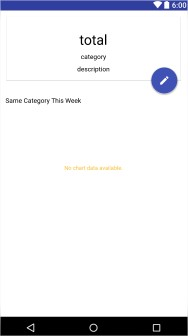
\includegraphics[width=5cm]{Chapter3/fragment.jpg}
	\caption{Expense Detail Fragment layout}
	\label{fig:Expense Detail Fragment layout}
\end{figure}
Since fragments can be attached or detached from an activity, there also exist onAttach() and onDetach() methods which are located in the MainFragment class in Spending Tracker app. After the fragment has been attached,can be used getActivity() within the fragment to get to the enclosing activity.This can be observed inside the \textit{onClick()} method in the Expenses Fragment class.
\begin{lstlisting}[caption={Getting to the enclosing activity},label={Getting to the enclosing activity},language = Java]
public void onClick(RecyclerView.ViewHolder vh, int position) {
	if (!expenseContainerListener.isActionMode()) {
		Expense expenseSelected = (Expense) vh.itemView.getTag();
		Intent expenseDetail = new Intent(getActivity(), ExpenseDetailActivity.class);
		expenseDetail.putExtra(ExpenseDetailFragment.EXPENSE_ID_KEY, expenseSelected.getId());
		startActivity(expenseDetail);
	} else {
		toggleSelection(position);
}
\end{lstlisting}
The same it works for all other fragments in the project.
\paragraph{Adding a fragment to an activity}\mbox{}\\
There are two ways of adding a fragment to the activity layout, such as a fragment contributes a portion of UI to the host activity, which is embedded as a part of the activity's overall view hierarchy.
\begin{itemize}
	\item Declare the fragment inside the activity's layout file.
	\item Or, programmatically add the fragment to an existing ViewGroup.
\end{itemize}
In the Spending Tracker application was used the second way.To make fragment transaction in the activity (such as add, remove, or replace a fragment), the APIs from FragmentTransaction must be used.The instance of FragmentTransaction from the Activity was obtained in the \textit{replaceFragment()} method like this:
\begin{lstlisting}[caption={Instance of Fragment Transaction},label={Instance of Fragment Transaction},language = Java]
public void replaceFragment(int containerId, Fragment fragment, boolean addToBackStack) {
	FragmentTransaction transaction = getSupportFragmentManager().beginTransaction();
	String tag = fragment.getClass().getSimpleName();
	transaction.replace(containerId, fragment, tag);
	if(addToBackStack) transaction.addToBackStack(null);
	transaction.commit();
}
\end{lstlisting}
The Fragment is replaced then in another method which has the same name,specifying the fragment to add and the view in which to insert it.
\begin{lstlisting}[caption={Fragment replacing},label={Fragment replacing},language = Java]
public void replaceFragment(Fragment fragment, boolean addToBackStack) {
	replaceFragment(R.id.main_content, fragment, addToBackStack);
}
\end{lstlisting}
By calling addToBackStack(), the replace transaction is saved to the back stack so the user can reverse the transaction and bring back the previous fragment by pressing the Back button.
Once the changes with FragmentTransaction were made, commit() must be called for the changes to take effect.

\subsubsection{Activities}
The Activities are crucial components of an Android application.Generally, one activity implements one screen in an app.Most apps contain multiple screens, which means they comprise multiple activities as happens in Spending Tracker application as well.
For the app to be able to use activities,the activities and certain of their attributes must be declared in the manifest.For example,here are declared two activities from Spending Tracker app:
\begin{lstlisting}[caption={AndroidManifest.xml},label={AndroidManifest.xml},language = XML]
<activity
	android:name=".ui.login.LoginActivity"
	android:configChanges="orientation"
	android:label="@string/app_name"
	android:screenOrientation="portrait"
	android:theme="@style/AppTheme.NoActionBar.TransparentStatusBar" >
	<intent-filter>
 		<action android:name="android.intent.action.MAIN" />
		<category android:name="android.intent.category.LAUNCHER" />
	</intent-filter>
</activity>
<activity android:name=".OcrCaptureActivity">
	<intent-filter>
		<category android:name="android.intent.category.LAUNCHER"/>
	</intent-filter>
</activity>
\end{lstlisting}
The only required attribute for this element is android:name, which specifies the class name of the activity. The rest of attributes define activity characteristics such as label, icon, or UI theme.There are also implicit requests which are declared using \textbf{<intent-filter>} attribute, in the \textbf{<activity>} element.The definition of this element includes an \textbf{<action>} element and, optionally, a \textbf{<category>} element.These elements combine to specify the type of intent to which your activity can respond.In the above example from Spending Tracker, for the first activity \textbf{android.intent.action.MAIN} means that this activity is the entry point of the application,when the application is launched, this activity is created.Category parameter gives additional information about the action to execute,\textbf{category.LAUNCHER} means it should appear in the Launcher as a top-level application.

Over its lifetime,an activity goes through a number of states.A series of callbacks can be used for handling transactions between states,such as are: onCreate(), onStart(), onResume(), onPause(),onStop(), onRestart(), onDestroy().The most trivial one is \textbf{onCreate()} callback.Bellow is presented an example from the MainActivity of Spending Tracker application.
\begin{lstlisting}[caption={onCreate() callback of MainActivity},label={onCreate() callback of MainActivity},language = Java]
protected void onCreate(Bundle savedInstanceState) {
	super.onCreate(savedInstanceState);
	setContentView(R.layout.activity_main);
	initUI();
	setUpDrawer();
	setUpToolbar();
	if ( savedInstanceState != null) {
		int menuItemId = savedInstanceState.getInt(NAVIGATION_POSITION);
		mainNavigationView.setCheckedItem(menuItemId);
		mainNavigationView.getMenu().performIdentifierAction(menuItemId, 0);
	} else {
		mainNavigationView.getMenu().performIdentifierAction(R.id.nav_expenses, 0);
	}
}
\end{lstlisting}
This callback must be implemented,it fires when system creates the activity.This callback initializes the essential components of the activity.This is where \textbf{setContentView()} must be called to define the layout for the  activity's user interface.
\subsection{Optical Character Recognition on Android – OCR}
Android can perform OCR very efficiently and correctly using the official Optical Character Recognition API of Android and the Mobile Vision library.Google has introduced recently \textbf{Mobile Vision APIs} \cite{MVAPIs}, which provide a very easy to use programming interfaces through which can be scanned Faces, Barcodes,QR Codes and Text without writing huge amount of code.And the best part is that these can be used offline as well.To enable the application to use Mobile Vision APIs, this dependency is needed to be added in the build.gradle file:
\[compile 'com.google.android.gms:play-services-vision:9.4.0+'\]
\paragraph{Introducing an Android OCR Library – Text Recognition API}\mbox{}\\
This Google powered API contains features like multiple language recognition,the Text API recognize text in any Latin based language. Also the text can be parsed from a stream of frames i.e. a video and displayed on the screen in real time.In Spending Tracker application the things are kept simple and the text is scanned from the photo of the receipt.All this is done offline by the Google Play services itself, i.e. no internet connection is required after once it has been set up in the application.
The Text Recognizer segments text into blocks, lines, and words.
\begin{itemize}
	\item a \textbf{Block} is a contiguous set of text lines, such as a paragraph or column;
	\item a \textbf{Line} is a contiguous set of words on the same vertical axis;
	\item a \textbf{Word} is a contiguous set of alphanumeric characters on the same vertical axis
\end{itemize}
Bellow is represented an example of each of these in descending order:
\begin{figure}[H]
	\centering
	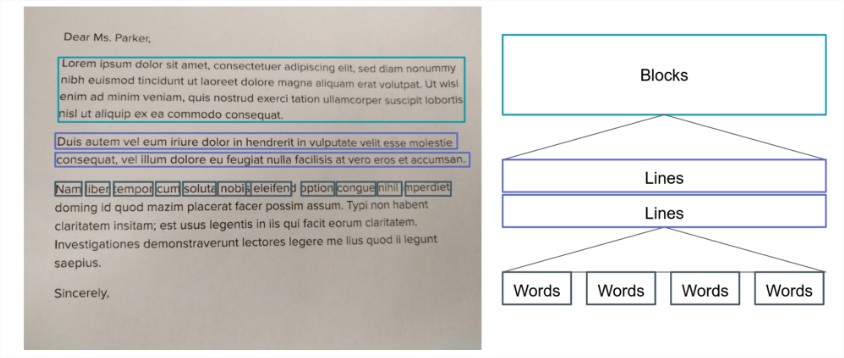
\includegraphics[width=16cm]{Chapter3/ocrex.jpg}
	\caption{Text Recognizer Example \cite{Text Recognition API}}
	\label{fig:Text Recognizer Example}
\end{figure}
\subsubsection{Tesseract library}
\subsubsection{Easy OCR library}
\subsection{User’s experience handling the product}
